\documentclass[border=2pt]{standalone}

% Required packages
\usepackage{amsmath}
\usepackage{amsfonts}
\usepackage{amssymb}
\usepackage{tikz}
\usepackage{tikz-cd}

% Load TikZ libraries
\usetikzlibrary{
    positioning,
    shapes,
    arrows.meta,
    calc,
    patterns,
    decorations.markings,
    cd
}

% Load custom styles
\usepackage{DZG-TikZ-Styles}

% Additional configurations
\tikzset{
    > = {Stealth[length=2mm, width=2mm]},
}

\begin{document}

% TikZ Diagram from V4 Thesis
% Source: writing/sources/enriques_paper/V2.tex
% Type: tikzpicture
% Category: general
% Index: 1

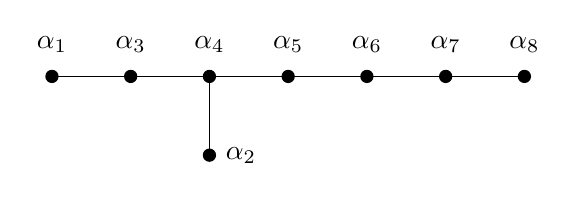
\begin{tikzpicture}
\draw  (0,0)-- (1,0);
\draw  (1,0)-- (2,0);
\draw  (2,0)-- (3,0);
\draw  (3,0)-- (4,0);
\draw  (4,0)-- (5,0);
\draw  (5,0)-- (6,0);
\draw  (2,0)-- (2,-1);

\fill [color=black] (0,0) circle (2.4pt);
\fill [color=black] (1,0) circle (2.4pt);
\fill [color=black] (2,0) circle (2.4pt);
\fill [color=black] (3,0) circle (2.4pt);
\fill [color=black] (4,0) circle (2.4pt);
\fill [color=black] (5,0) circle (2.4pt);
\fill [color=black] (6,0) circle (2.4pt);
\fill [color=black] (2,-1) circle (2.4pt);

\draw[color=black] (2.4,-1) node {$\alpha_2$};
\draw[color=black] (0,0.4) node {$\alpha_1$};
\draw[color=black] (1,0.4) node {$\alpha_3$};
\draw[color=black] (2,0.4) node {$\alpha_4$};
\draw[color=black] (3,0.4) node {$\alpha_5$};
\draw[color=black] (4,0.4) node {$\alpha_6$};
\draw[color=black] (5,0.4) node {$\alpha_7$};
\draw[color=black] (6,0.4) node {$\alpha_8$};
\end{tikzpicture}


\end{document}
